\documentclass[11pt, oneside]{article} 
\usepackage[margin=3.4cm]{geometry} 
\geometry{letterpaper}
\usepackage{graphicx}
\usepackage{hyperref}
\usepackage{amssymb}
\usepackage{caption}
\usepackage{float}
\usepackage{setspace}
\usepackage{esvect}
\usepackage{url}
\usepackage[section]{placeins}
\usepackage{multirow}
\usepackage{amsmath}
\usepackage{array}
\usepackage{adjustbox}

%\setcounter{secnumdepth}{0}
\onehalfspacing

\newcounter{refno}
\newcommand{\reflabel}[1]{\refstepcounter{refno}\label{#1}[\arabic{refno}]}  %create ref labels in-text

\newcommand{\refinit}[1]{\noindent \hangindent=0.6cm [\ref*{#1}]}  %citation initialization in reference section

\begin{document}
% Title Page
\begin{titlepage}
	\newcommand{\HRule}{\rule{\linewidth}{0.5mm}}
	
	\center
	\textsc{\LARGE University of Calgary}\\[1.5cm]
	\textsc{\Large ENGO 651: Advanced Geospatial Topics}\\[0.5cm]
	\textsc{\large Final Project}\\[0.5cm]

	\HRule\\[0.4cm]
	{\huge\bfseries Fuellytics: Real-Time Vehicular Fuel Consumption and Emissions Monitoring}\\[0.4cm]
	\HRule\\[1.5cm]
	
	{\large\textit{Group 2}}\\
	Adam \textsc{Smith} (30031453)\\
	Chavisa \textsc{Sornsakul} (30193209)\\
	Wai Ka \textsc{Wong Situ} (30184219)\\
	
	\vfill\vfill\vfill
	{\large \today}
	
	\vfill\vfill\vfill
	
\includegraphics[width=8cm,]{img/schulich.png}\\[1cm]	
\end{titlepage}

\section{Executive summary}
Next to oil and gas, the transportation sector is the second largest emitter of greenhouse gases in Canada.  Since 1990, Canadian greenhouse gas emissions from transportation have increased by over 32\%, and this is largely driven by increases from passenger vehicles \reflabel{canadaghg}.  Mitigating these emissions is crucial to reducing the harmful effects of climate change on the environment and protecting our natural landscapes.

Monitoring fuel consumption is vital to understand the efficiency of a vehicle and its impact on the environment.  This data can provide valuable insights into the effects of driving style, conditions, and vehicle type on a vehicle's emissions, and incentivize the driver to adapt their driving style to reduce total greenhouse gas emissions and fuel costs.  

Our innovative new smartphone application, \textit{Fuellytics}, utilizes the smartphone's inertial, magnetic, and GNSS sensors to measure fuel consumption and emissions of various greenhouse gases in real-time.  Fuellytics helps drivers track their fuel costs by monitoring velocity and acceleration while driving, and displaying the current and total fuel use for the current trip on an interactive frontend.  Moreover, the user is able to track their routes, and analyze their CO$_2$ emissions on current and previous routes.

The dynamic frontend of Fuellytics is built using the JavaScript library React-Native \reflabel{reactnative} to enable simplified development and cross-platform compatibility.  To alllow for easy user authentication and provide versatile development tools, the backend is written with the Python library Django \reflabel{django}.

Fuellytics uses various AWS \reflabel{aws} services, including an elastic load balancer, sticky sessions, EC2 instances, security groups, auto-scaling groups, AWS RDS, S3 bucket, and Lambda serverless function to provide a scalable and reliable platform. The application uses the WebSocket protocol to connect to the Lambda serverless function for real-time data processing using sensor fusion techniques. CloudWatch is used for monitoring and logging every action or error in run-time as well as build-time. The application is created to meet the needs of its users while emphasizing reliability and scalability.

This report discusses in detail the motivation, proposed solution, and implementation of the Fuellytics application.  Section 2 outlines the problem statement, and the Fuellytics solution is proposed in section 4.  In section 3, a literature review is conducted on the available literature and similar solutions and their differences with the proposed application are discussed.  Section 5 outlines the application architecture and the design rationale.  A description of the results is presented in section 6, lessons learned are discussed in section 7, and the report in concluded in section 8.

\section{Problem statement}
According to the International Energy Agency, transportation accounts for almost one-quarter of global greenhouse gas emissions, and within that, road transport is responsible for the largest share of emissions \reflabel{transport-emissions}.  The burning of fossil fuels in vehicles produces, along with several other pollutants, carbon dioxide, which is the most prevalent greenhouse gas contributing to global warming.  Although electric vehicles are becoming more popular in the developed world, still 91\% of all transport relies on oil-based products such as gasoline, which is only a 3\% drop from the early 1970's \reflabel{oil-based-transport}.  Reducing carbon emissions from vehicles is crucial to mitigate the harmful effects of climate change and reduce the environmental burden of vehicular transport.

Tracking vehicle fuel consumption is essential to understanding the amount of carbon emissions produced by vehicles. Fuel consumption data can provide valuable insights into the efficiency of a vehicle and its impact on the environment, and can also provide insights to the driver about their driving style and fuel costs.  However, fuel consumption is heavily dependent on various factors such as vehicle type, terrain, and driving style, making it difficult to measure over short time periods.  According to the US Department of Energy, obeying speed limits, accelerating and braking gently, and reading the road ahead can improve fuel economy by up to 30\% on highways and up to 40\% in stop-and-go traffic \reflabel{driving-style}.  Moreover, engine size, vehicle weight, and driving in hilly or mountainous areas can drastically increase fuel consumption and, consequently, carbon emissions.  Some modern vehicles are equipped with a dashboard gauge that displays fuel consumption while driving, however, these gauges are often vague and uninformative, usually showing nothing more than an unlabelled bar or dial which increases while accelerating.  Without a means to directly monitor fuel consumption, drivers are often left unaware of their fuel use and how their driving style and driving conditions can be altered to reduce their vehicle's impact on the environment.

The presented smartphone application, \textit{Fuellytics}, provides an innovative solution to monitoring fuel consumption and greenhouse gas emissions in real-time, and provides insights and reports to drivers about their fuel use while driving as well on previous trips.  Fuellytics helps drivers better understand the environmental impacts of their vehicle, make educated decisions regarding transportation, and save money on fuel.

\section{Similar solutions and available literature}

For industrial applications, several fleet management solutions exist that offer analytics on fuel consumption and tracking.  For example, \textit{FuelForce Fuel Management Systems} \reflabel{fuel-force} provides tools to monitor, track, view, and analyze fuel use of fleet vehicles, and \textit{Triscan} \reflabel{triscan} provides a similar functionality by integrating their systems with refuelling stations. These solutions, however, are targeted at industrial applications, and do not provide real-time analytics to the driver.  Moreover, these and similar tools are focused around fleet management and cost savings, and often do not provide an analysis of environmental impact.

Multiple applications for personal use exist which track fuel usage over long periods of time to determine fuel costs and fuel economy. The web and iOS application \textit{Fuelly} \reflabel{fuelly} allows users to enter volume and cost data each time they refuel to gain insight into their fuel consumption and fuel costs over time.  A similar application, \textit{FuelLine} \reflabel{fuelline}, was recently developed by a team at BCIT and additionally contains a routing feature to predict fuel costs on future routes.  Notably, these solutions differ from Fuellytics in that they do not provide real-time fuel consumption data while driving and they are focused more on monitoring costs rather than reducing environmental impacts.

Some applications developed for carbon emission tracking, such as \textit{MyEarth} \reflabel{myearth} and \textit{Carbon Footprint \& CO2 Tracker} \reflabel{capture}, provide functionality to track CO$_2$ emission in many categories including travel.  However, the main focus of these applications is tracking carbon emissions in a broad range of categories, not an in-depth and real-time analysis of carbon emissions and fuel use from driving.

A 2019 paper \reflabel{main-paper} from the North China University of Technology utilized the vehicle specific power (VSP) distribution to predict fuel consumption in real-time from velocity and acceleration data using a binned linear regression approach.  Their model achieves a relatively low error while requiring only velocity, acceleration, engine displacement, and the presence or absence of a supercharger or turbocharger as input.  However, the road surface is assumed flat, so road gradient is not included in the model.

\reflabel{tank2wheel} and \reflabel{analytic-fc} both derive more sophisticated models for the real-time fuel consumption and emissions of light-duty vehicles.  These models provide more accurate results than the model described in [\ref*{main-paper}], but require knowledge of many parameters specific to the vehicle such as rotational internal inertia of the engine, the selected gear, the tire radius, and the total loaded weight.  These parameters are generally unknowable in our application.  Other methods, such as those described in \reflabel{wvu-ai} and \reflabel{fc-phone}, compute fuel consumption post-trip using various methods, but lack a real-time fuel consumption analysis, so are unsuitable for our application.

As such, Fuellytics uses an adaptation of the method described in [\ref*{main-paper}] as the basis for the numerical prediction of real-time fuel consumption.  This model was chosen due to its simplicity, relatively low error, and availability of the model parameters.  Modification of the model to account for road gradient is also easily implemented.

\section{Solution summary}

Our innovative application, \textit{Fuellytics}, is a cutting-edge smartphone application that enables drivers of light-duty passenger vehicles to track their fuel consumption and CO$_2$ equivalent emissions in real-time.  After creating an account and registering their vehicle, users can log their trips, and the app collects data on location, acceleration, and angular velocity from the sensors embedded in the smartphone while driving.  Fuellytics utilizes this data to compute the rates of fuel consumption and pollutant production and displays this information in an interactive user interface to provide insights regarding the user's fuel use and environmental impact. 

The application not only displays emissions and fuel consumption information, but also tracks their current location and displays their trip on an interactive map.  Furthermore, the user can view and analyze fuel consumption and CO$_2$ emissions from previously logged trips, and see their previous routes on a map. These statistics allow users make educated decisions about their driving and transportation habits and adjust their driving style to improve fuel economy and save money.  Moreover, they highlight the environmental impact of their vehicle use to promote environmentally friendly transportation choices.

\section{Architecture}

\subsection{Architecture description and design rationale}

Our application is built using several AWS services that work together to provide a scalable and reliable platform. The main entry point is the elastic load balancer, responsible for balancing and distributing user traffic evenly. To ensure the user doesn't lose their session, sticky sessions are applied here. EC2 instances are connected to the load balancer via security groups, which act as firewalls to prevent access from entry points other than the load balancer.

To handle scaling based on usage or pre-defined metrics such as CPU performance or scheduled events, the EC2 instances are contained within an auto-scaling group. AWS RDS, specifically Postgresql DB, is used to store critical data for the application. Alternative choices include Amazon Aurora and DynamoDB (NoSQL). Static files such as profile and car images are stored in an S3 bucket, which acts as a CDN and is connected to the EC2 instances. CloudFront implementation can be used to further scale for high availability.

When the user starts recording, it connects to a lambda serverless function via API Gateway using the WebSocket protocol. The client's device streams accelerometer, gyroscope, magnetometer, and GPS data to the lambda function, which processes the data using sensor fusion and the Madgwick AHRS algorithm \reflabel{madgwick} to return real-time metrics shown directly to the user. It's worth noting that the limitation of the serverless function comes from cold starts, meaning the initial connection may be slower than subsequent ones.

Once the user completes a trip, the client sends a POST request with all the client-stored data to the backend. For monitoring, we are employing CloudWatch, which logs every action or error in run time as well as build time. With this combination of services, we have created a scalable, reliable, and efficient application that meets the needs of our users.

Figures \ref{fig:architecture} and \ref{fig:frontend} and Table \ref{table:backend} show diagrammatic representations of the architecture of the Fuellytics application.  The technologies used to develop Fuellytics are show in Figure \ref{fig:tech-stack}.

\begin{figure}[!htb]
\centerline{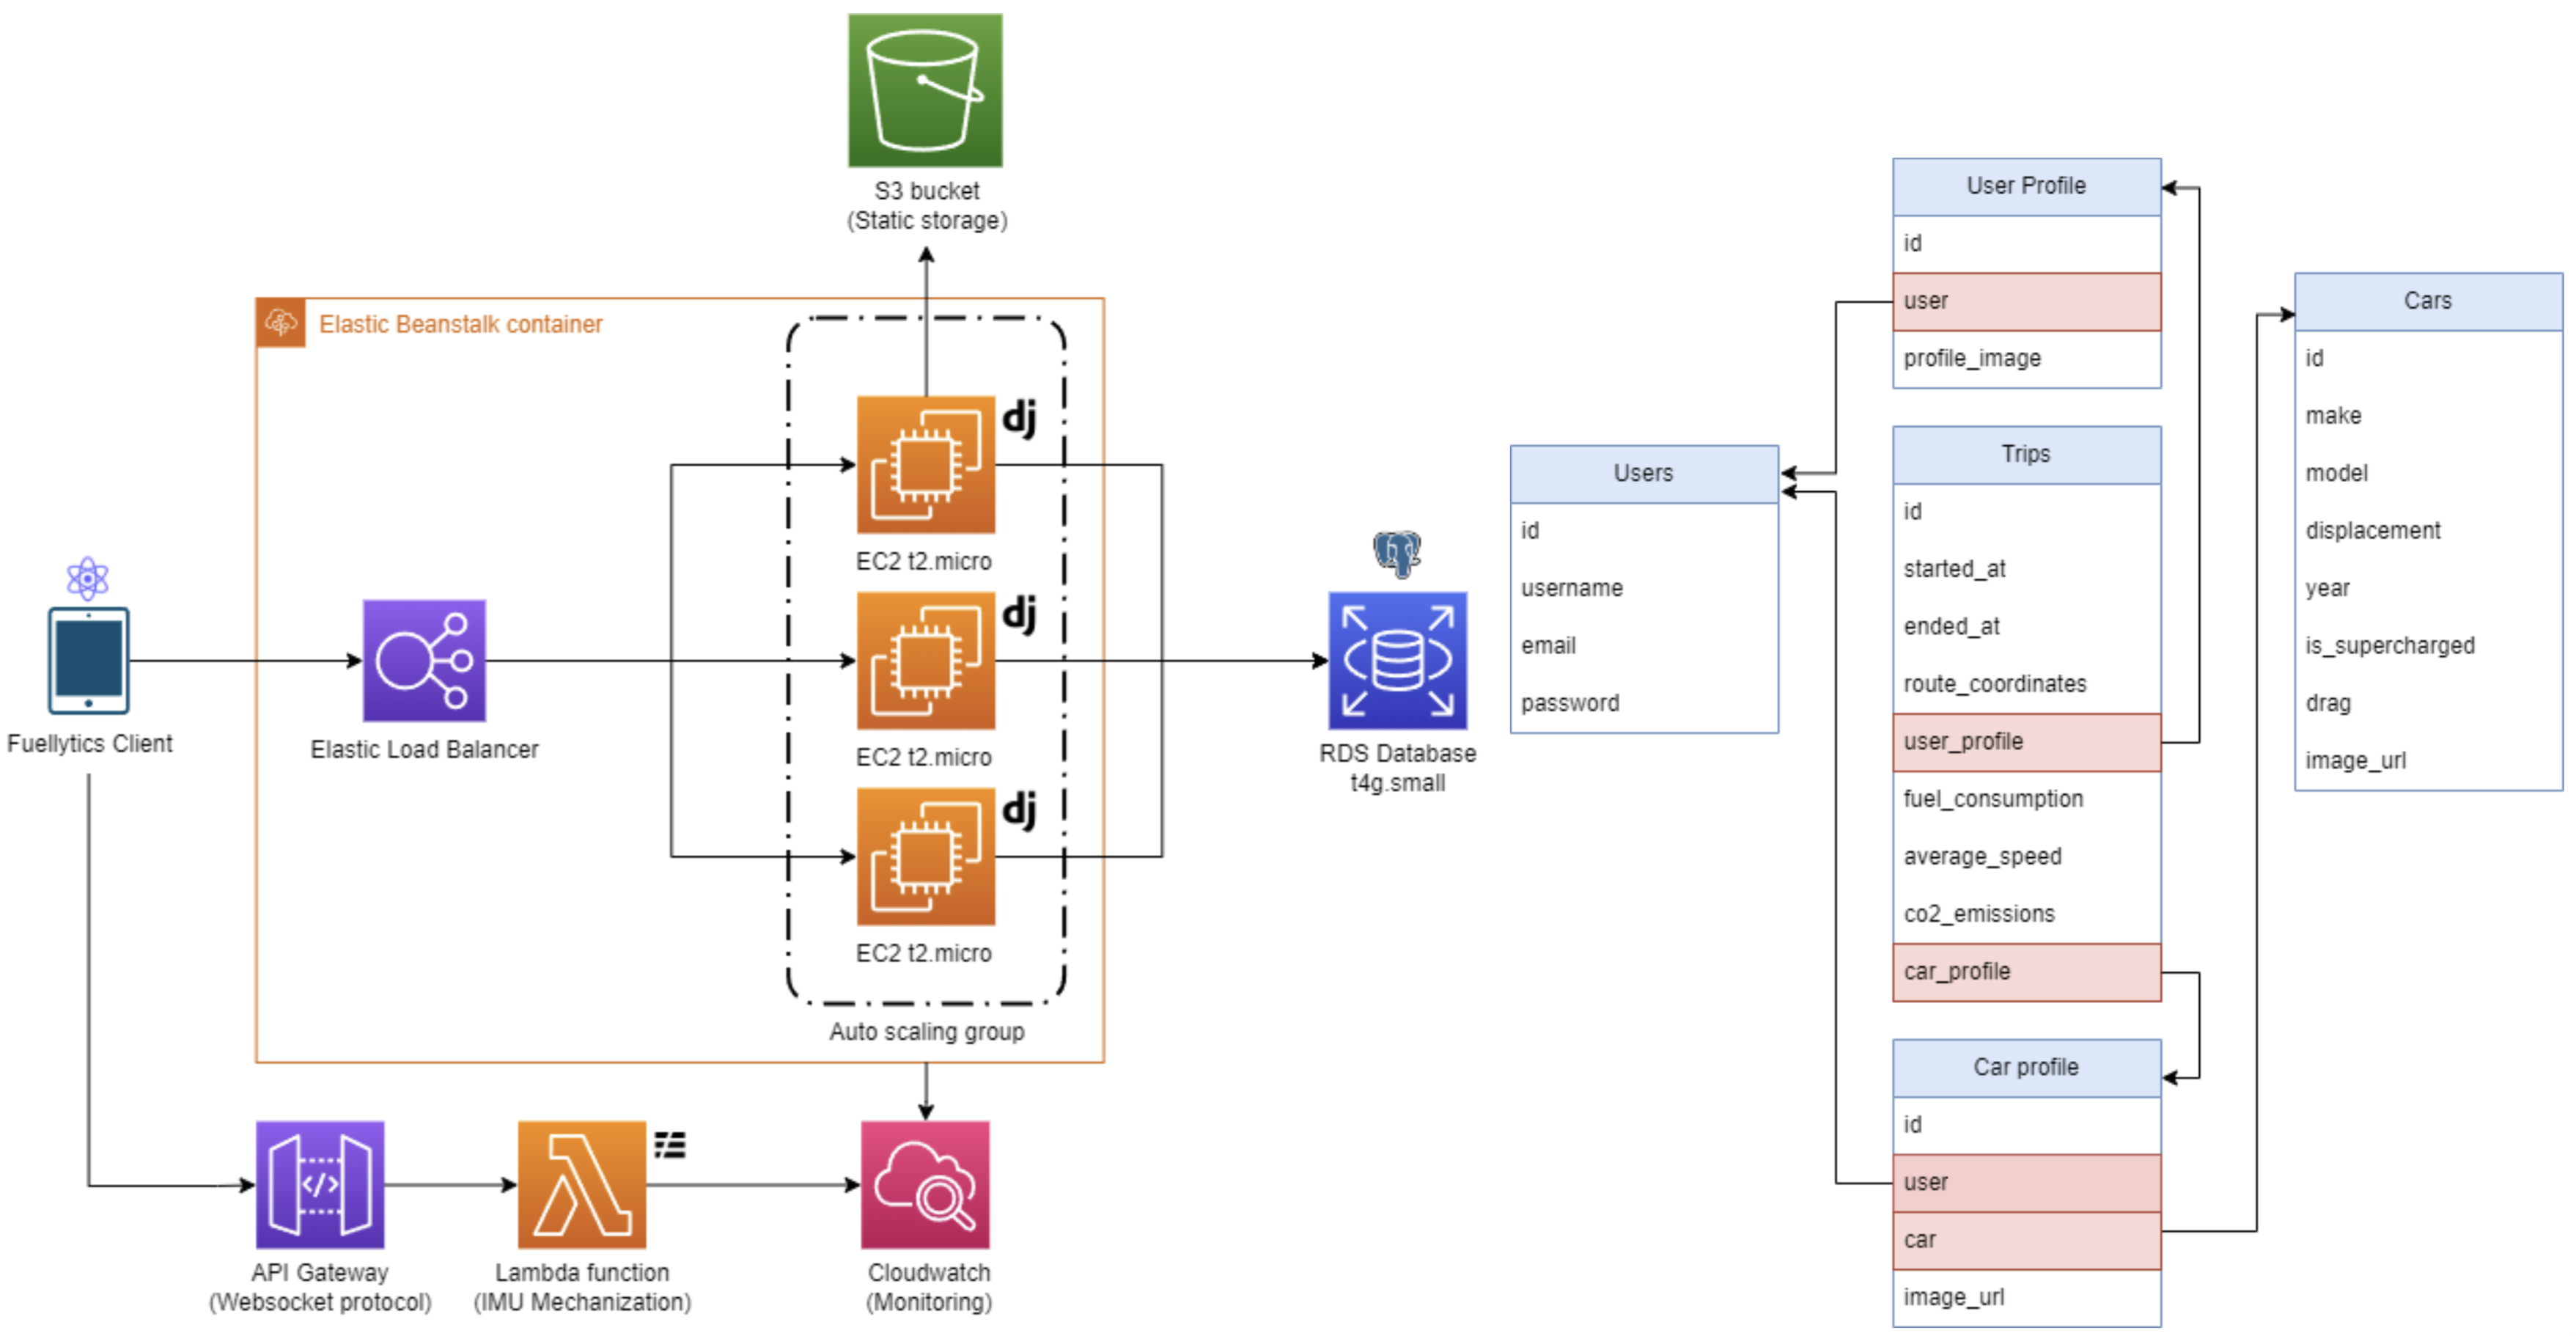
\includegraphics[width=19cm]{img/architecture/architecture-aws.png}}
\caption{\label{fig:architecture}Fuellytics applies the classic three-tier architecture (Client, Server, and DB) most commonly used among simple applications. The design is widely accepted by current industry standards due to its low complexity and high scalability potential.}
\end{figure}

\begin{figure}[!htb]
\centerline{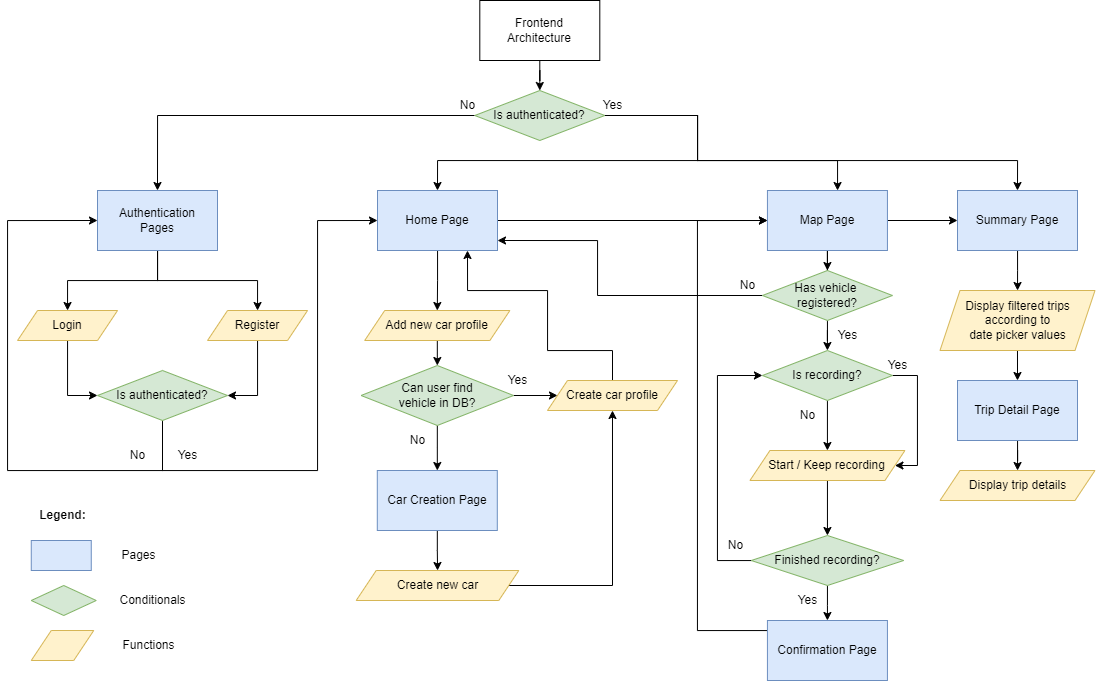
\includegraphics[width=17cm]{img/architecture/Fuellytics-Frontend Architecture.png}}
\caption{\label{fig:frontend}The frontend architecture consists of 4 main sections, authentication pages, home pages, map pages, and summary pages. Each section contains its own logic flow and subpages.}
\end{figure}

\begin{table}[!t]
\scriptsize
\renewcommand{\arraystretch}{1.275}
\vspace*{-1.5cm}
\centerline{\begin{tabular}{|c|c|c|c|c|c|}
\hline
\begin{adjustbox}{padding=1em}
\textbf{\small App}
\end{adjustbox} &
  \textbf{\small Description} &
  \textbf{\small Method} &
  \textbf{\small Endpoint} &
  \textbf{\small Parameters} &
  \textbf{\small Body} \\ \hline
\multirow{5}{*}{\begin{tabular}[c]{@{}c@{}}\vspace*{.25cm}\\User \end{tabular}} &
  \multirow{5}{*}{\begin{tabular}[c]{@{}c@{}}\vspace*{.25cm} \\Base Django user\\ model.\end{tabular}} &
  POST &
  /api/accounts/login &
  - &
  \begin{tabular}[c]{@{}c@{}}username: string\\ password: string\end{tabular} \\ \cline{3-6} 
 &
   &
  POST &
  /api/accounts/register &
  - &
  \begin{tabular}[c]{@{}c@{}}username: string\\ password: string\\ email: string\end{tabular} \\ \cline{3-6} 
 &
   &
  DELETE &
  /api/accounts/logout &
  - &
  - \\ \cline{3-6} 
 &
   &
  GET &
  /api/accounts/current\_user &
  - &
  - \\ \cline{3-6} 
 &
   &
  GET &
  /api/accounts/csrf\_cookie &
  - &
  - \\ \hline
User Profile &
  \begin{tabular}[c]{@{}c@{}}Include extra fields from\\ the user. The User Profile\\ app is connected to User\\ via a one-to-one\\ relationship.\end{tabular} &
  GET &
  /api/accounts/users/:id &
  - &
  - \\ \hline
\multirow{3}{*}{\begin{tabular}[c]{@{}c@{}}\vspace*{1.05cm} \\Cars \end{tabular}} &
  \multirow{3}{*}{\begin{tabular}[c]{@{}c@{}}\vspace*{.65cm} \\ Include the list of cars\\ that the user can select\\ from.\end{tabular}} &
  GET &
  /api/cars/ &
  \begin{tabular}[c]{@{}c@{}}search?: string\\ make?: string\\ model?: string\\ displacement?: number\\ year?: number\\ is\_supercharged?: boolean\end{tabular} &
  - \\ \cline{3-6} 
 &
   &
  GET &
  /api/cars/:id &
  - &
  - \\ \cline{3-6} 
 &
   &
  POST &
  /api/cars/ &
  - &
  \begin{tabular}[c]{@{}c@{}}make: string\\ model: string\\ displacement: string\\ year: number\\ is\_supercharged: boolean\\ drag: number\end{tabular} \\ \hline
\multirow{3}{*}{Car Profile} &
  \multirow{3}{*}{\begin{tabular}[c]{@{}c@{}}Relates the list of cars\\ owned by the user to\\ the user.\end{tabular}} &
  GET &
  /api/car\_profiles/ &
  user\_id?: number &
  - \\ \cline{3-6} 
 &
   &
  GET &
  /api/car\_profiles/:id &
  - &
  - \\ \cline{3-6} 
 &
   &
  POST &
  /api/car\_profiles/ &
  - &
  car\_id: number \\ \hline
\multirow{3}{*}{\begin{tabular}{@{}c@{}}\vspace*{2.5cm} \\Trips\end{tabular}} &
  \multirow{3}{*}{\begin{tabular}[c]{@{}c@{}}\vspace*{2.25cm}\\List of trips that the user\\has recorded.\end{tabular}} &
  GET &
  /api/trips/ &
  \begin{tabular}[c]{@{}c@{}}user\_id?: number\\ started\_at?: Date\\ ended\_at?: Date\end{tabular} &
  - \\ \cline{3-6} 
 &
   &
  GET &
  /api/trips/:id &
  - &
  - \\ \cline{3-6} 
 &
   &
  POST &
  /api/trips/ &
  - &
  \begin{tabular}[c]{@{}c@{}}started\_at: Date\\ ended\_at: Date\\ route\_coordinates: \{\\ latitude: number\\ longitude: number\\ speed: number\\ heading: number\\ altitude: number\\ accuracy: number\\ altitude\_accuracy: number\\ \}[\hspace*{.06cm}]\\ fuel\_consumption: number\\ average\_speed: number\\ co2\_emissions: number\end{tabular} \\ \hline
\end{tabular}}
\caption{\label{table:backend}The backend architecture and API documentation for the Fuellytics application.}
\end{table}

\begin{figure}[!htb]
\centerline{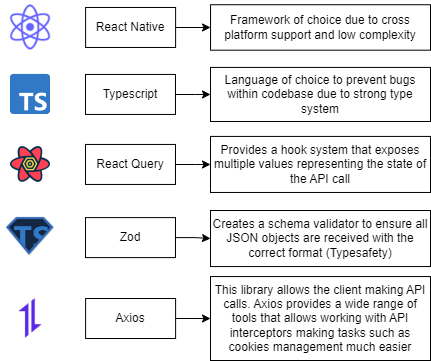
\includegraphics[width=9cm]{img/architecture/Fuellytics-Frontend Tech stack.png}}
\caption{\label{fig:tech-stack}The frontend tech stack employed in the Fuellytics application.}
\end{figure}

\FloatBarrier 
\subsection{Continuous integration/continuous delivery architecture}
Fuellytics is a multi-repo project, however, the CI/CD architecture, shown in Figure \ref{fig:cicd}, follows the same workflow delivery pattern in all three repositories. It starts with the developer creating a new branch from the protected master branch. When code changes are ready, they are collected into a pull request and the review process starts. Once all checks are cleared, the pull request is merged into the master branch and an automated-deployment pipeline builds and deploys the project into its respective infrastructure.

\begin{figure}[!htb]
\centerline{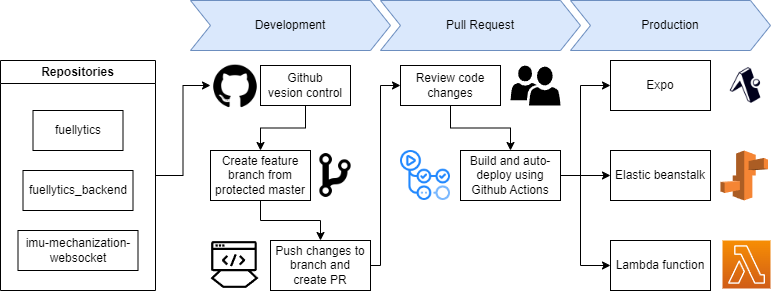
\includegraphics[width=15cm]{img/architecture/Fuellytics-CI_CD Workflow.png}}
\caption{\label{fig:cicd}CI/CD architecture of the Fuellytics application.}
\end{figure}

\section{Results}
Upon opening Fuellytics, the user is presented with a login page (Figure \ref{fig:login-register}) showing the Fuellytics logo and fields for the user to enter their credentials, as well as a login button. If the user attempts to login with invalid or missing credentials, the login attempt will fail.  A successful login will bring the user to the home page of the application.

If the user is not yet registered, they can select the register button to be brought to the registration page shown in Figure \ref{fig:login-register}.  To register, the user must provide a username (containing at most 150 characters) and email (with valid email formatting) which are not already associated with an account, and a password with a minimum length of 8 characters.  If these requirements are not met, the registration will fail. Upon successful registration, the user will automatically be logged in and brought to the application home page, shown in Figure \ref{fig:homepage}.
\begin{figure}[H]
\centerline{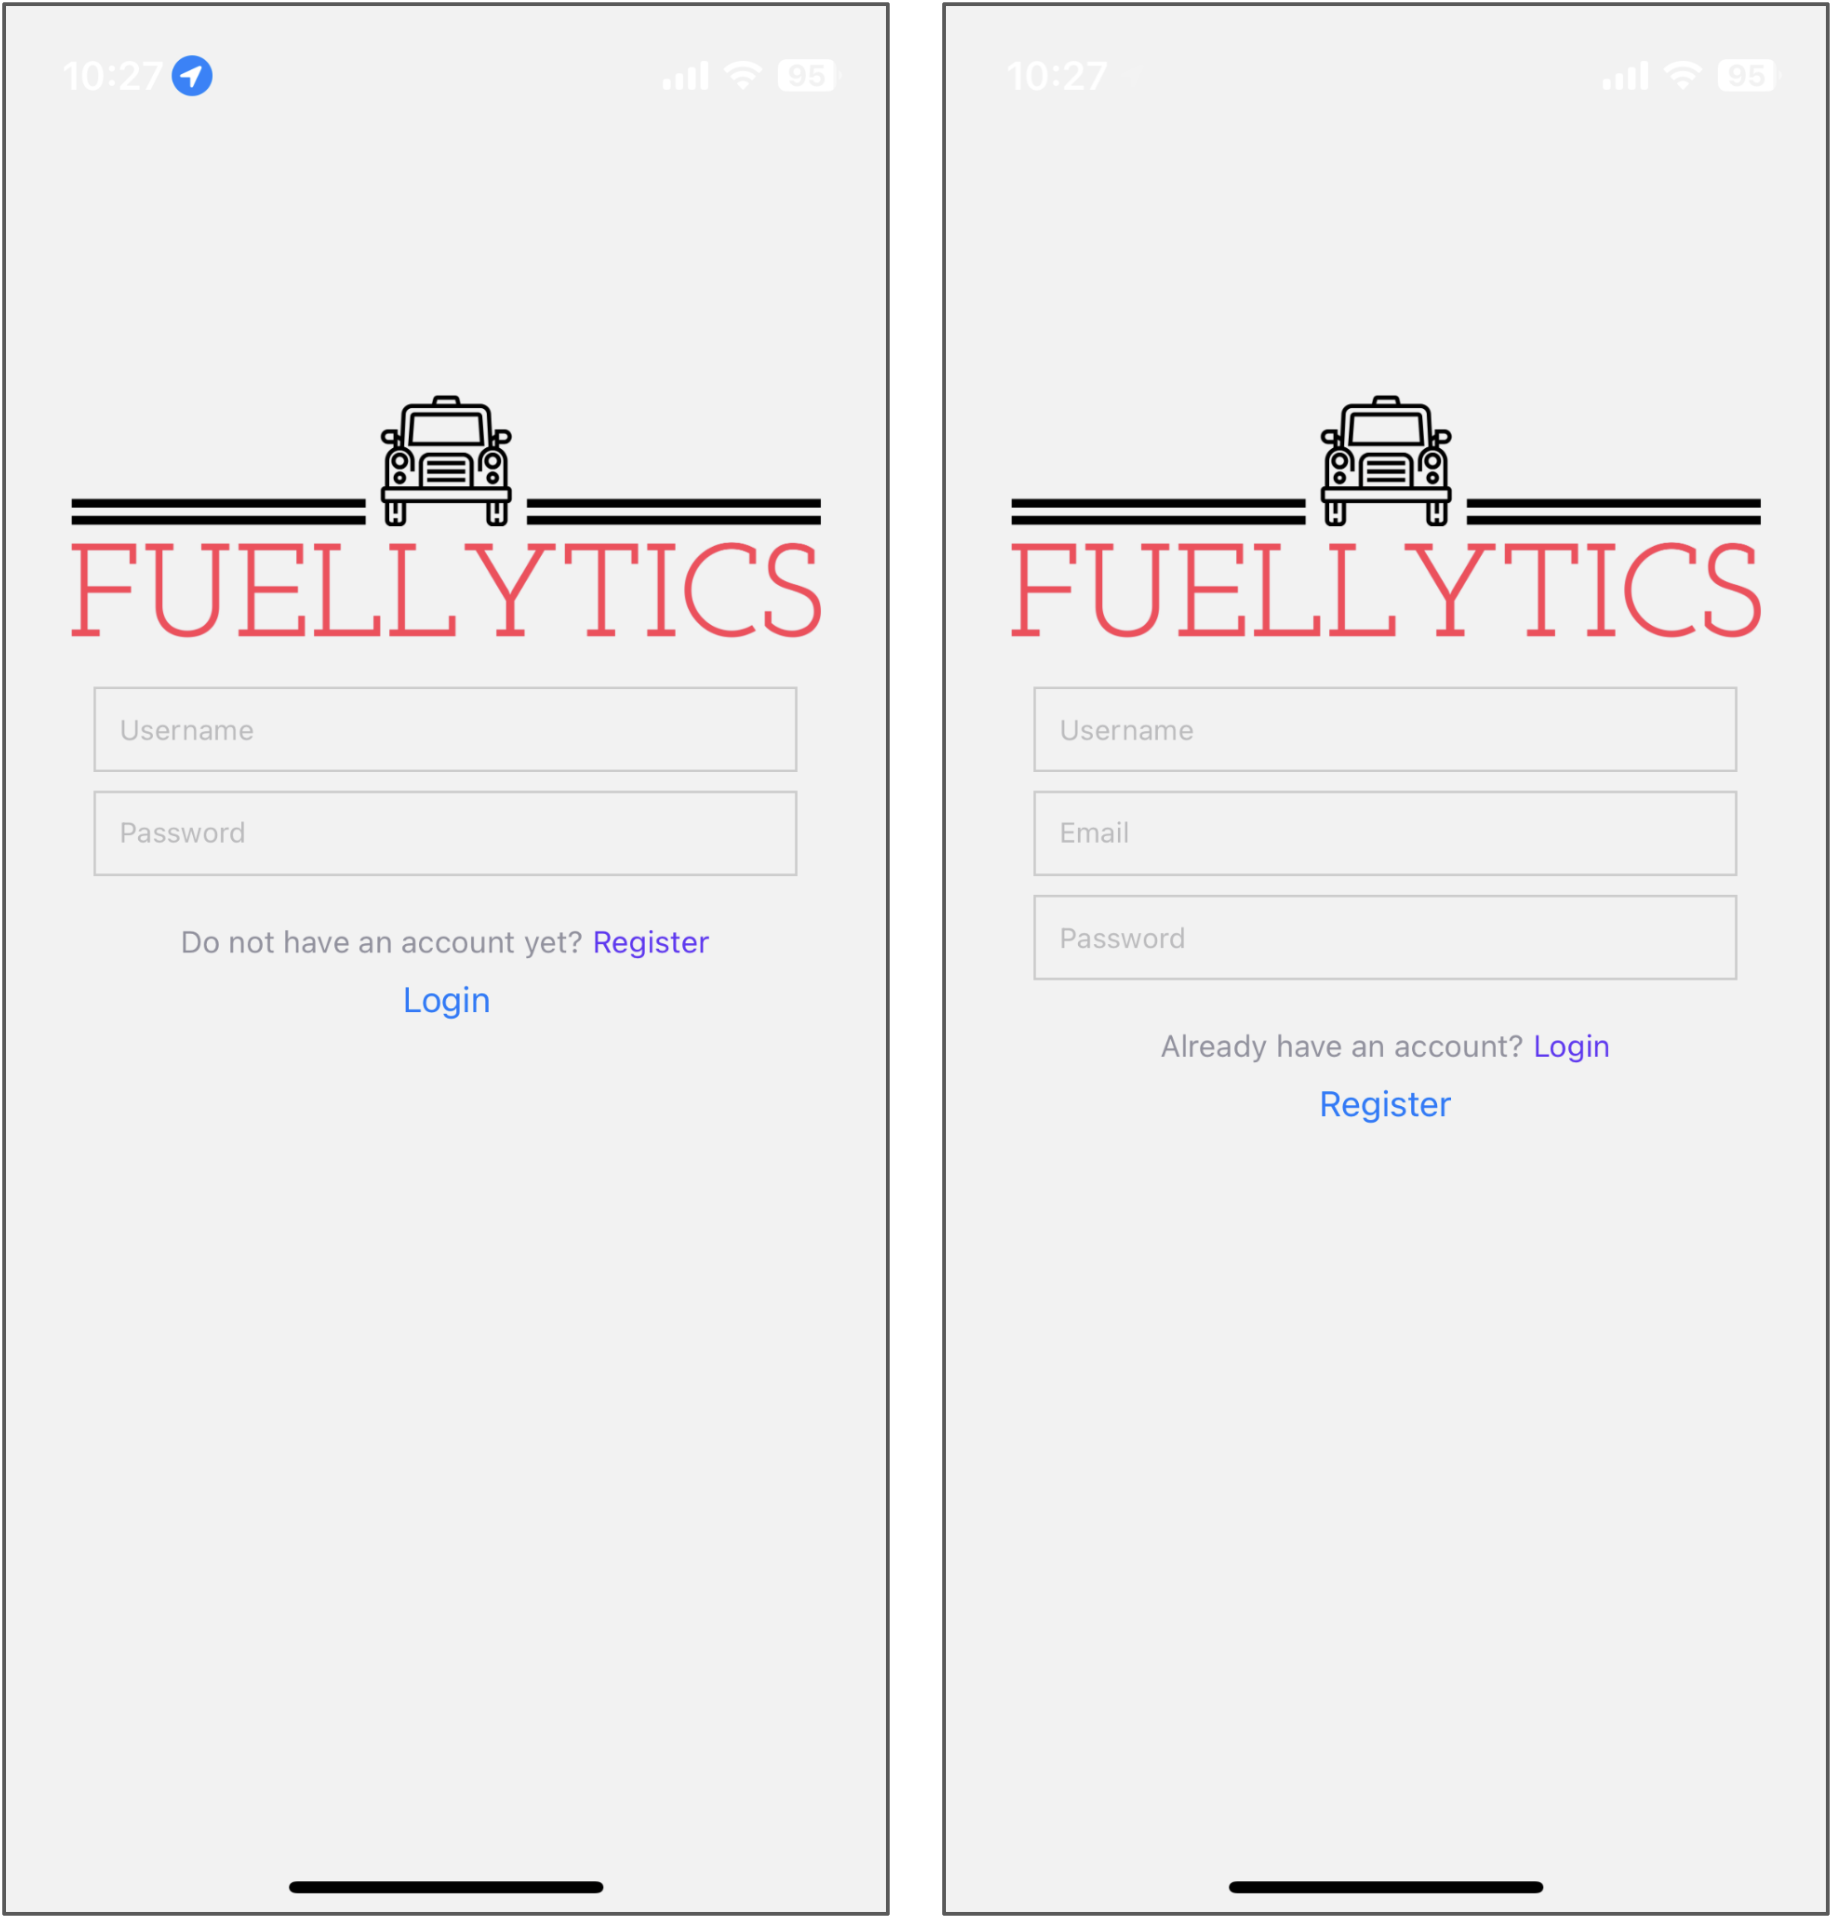
\includegraphics[width=11cm]{img/login-register.png}}
\caption{\label{fig:login-register}Login page (left) and registration page (right) of the Fuellytics application.}
\end{figure}

On the home page the user is greeted with a welcome message, and the list of vehicles that the user has added to their account is displayed.  If there are no vehicles associated with the user's account, the message ``No vehicles registered.'' is displayed.  A logout button is available in the top left corner of the page.

The user can easily remove vehicles by selecting the `x' icon next to the vehicle name. Vehicles can be added by selecting the ``Add new vehicle'' button above the navigation bar.  This brings up a popup (Figure \ref{fig:new-vehicle}) where the user can search for their vehicle by typing in the search field, and then create the vehicle profile by selecting the ``Create'' button.  Fuellytics has data for over 22,000 unique vehicles, however, if the user's vehicle is not available, the user can manually enter their vehicle's credentials after selecting the ``Enter my own vehicle'' button.  The credentials required by Fuellytics are the make, model, year, engine displacement, and whether or not the vehicle is supercharged.
\begin{figure}[H]
\centerline{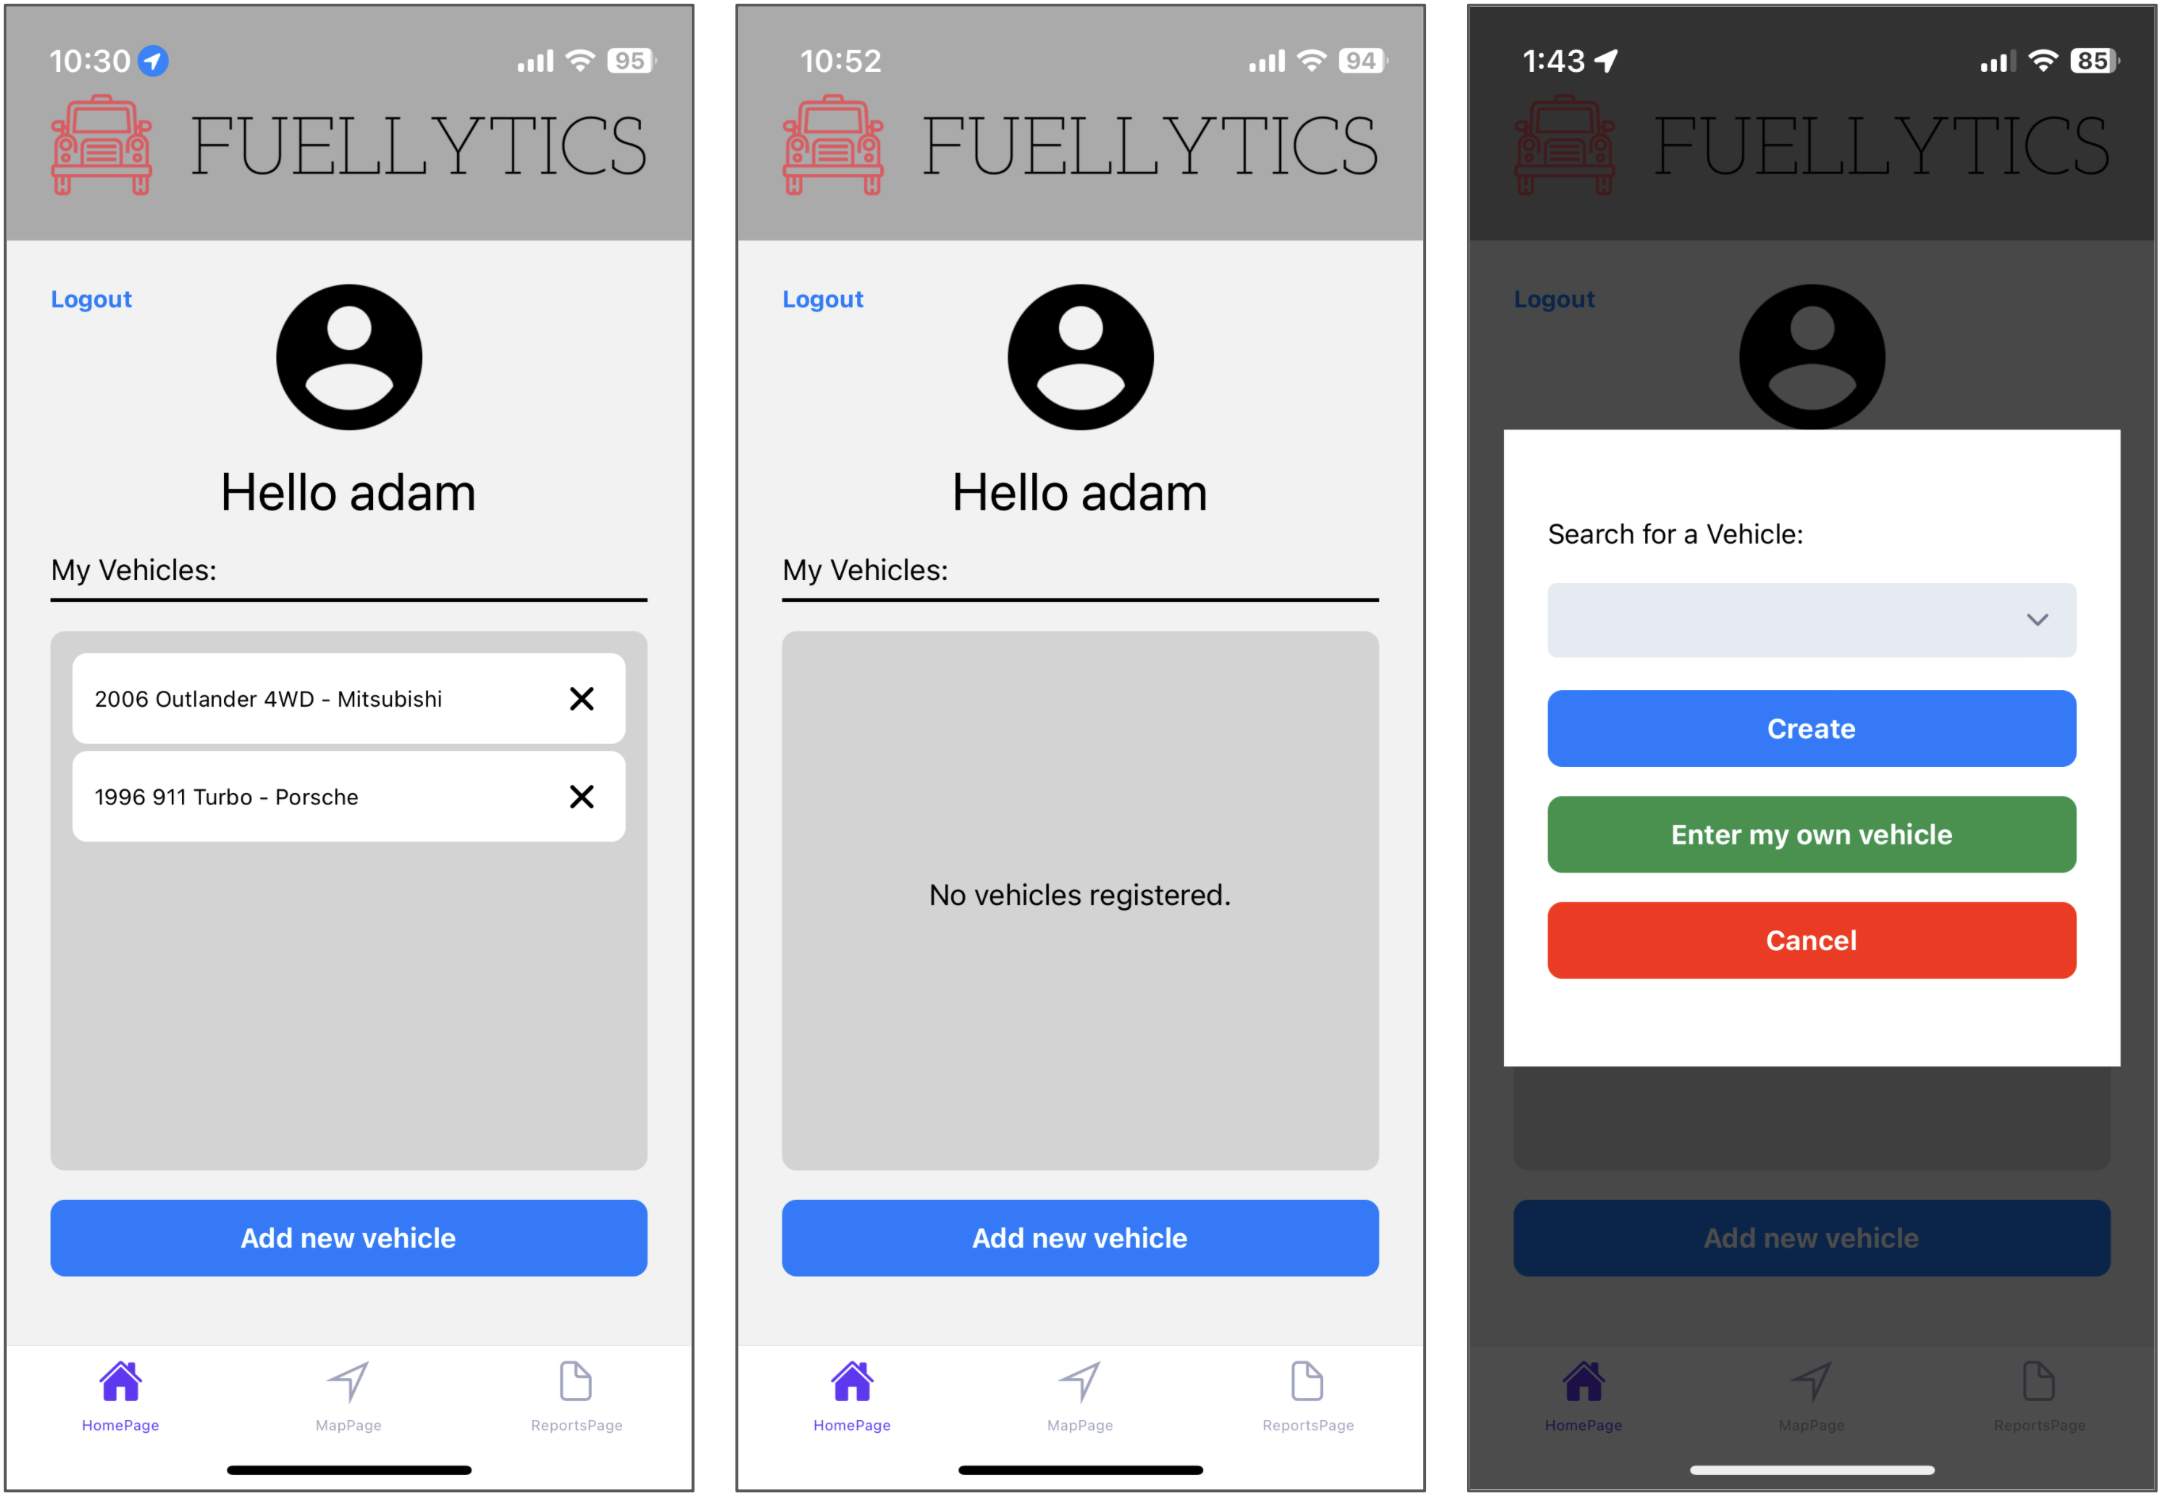
\includegraphics[width=11cm]{img/homepage.png}}
\caption{\label{fig:homepage}The Fuellytics home page with (left) and without (middle) vehicles added to the user's account.}
\end{figure}
\begin{figure}[H]
\centerline{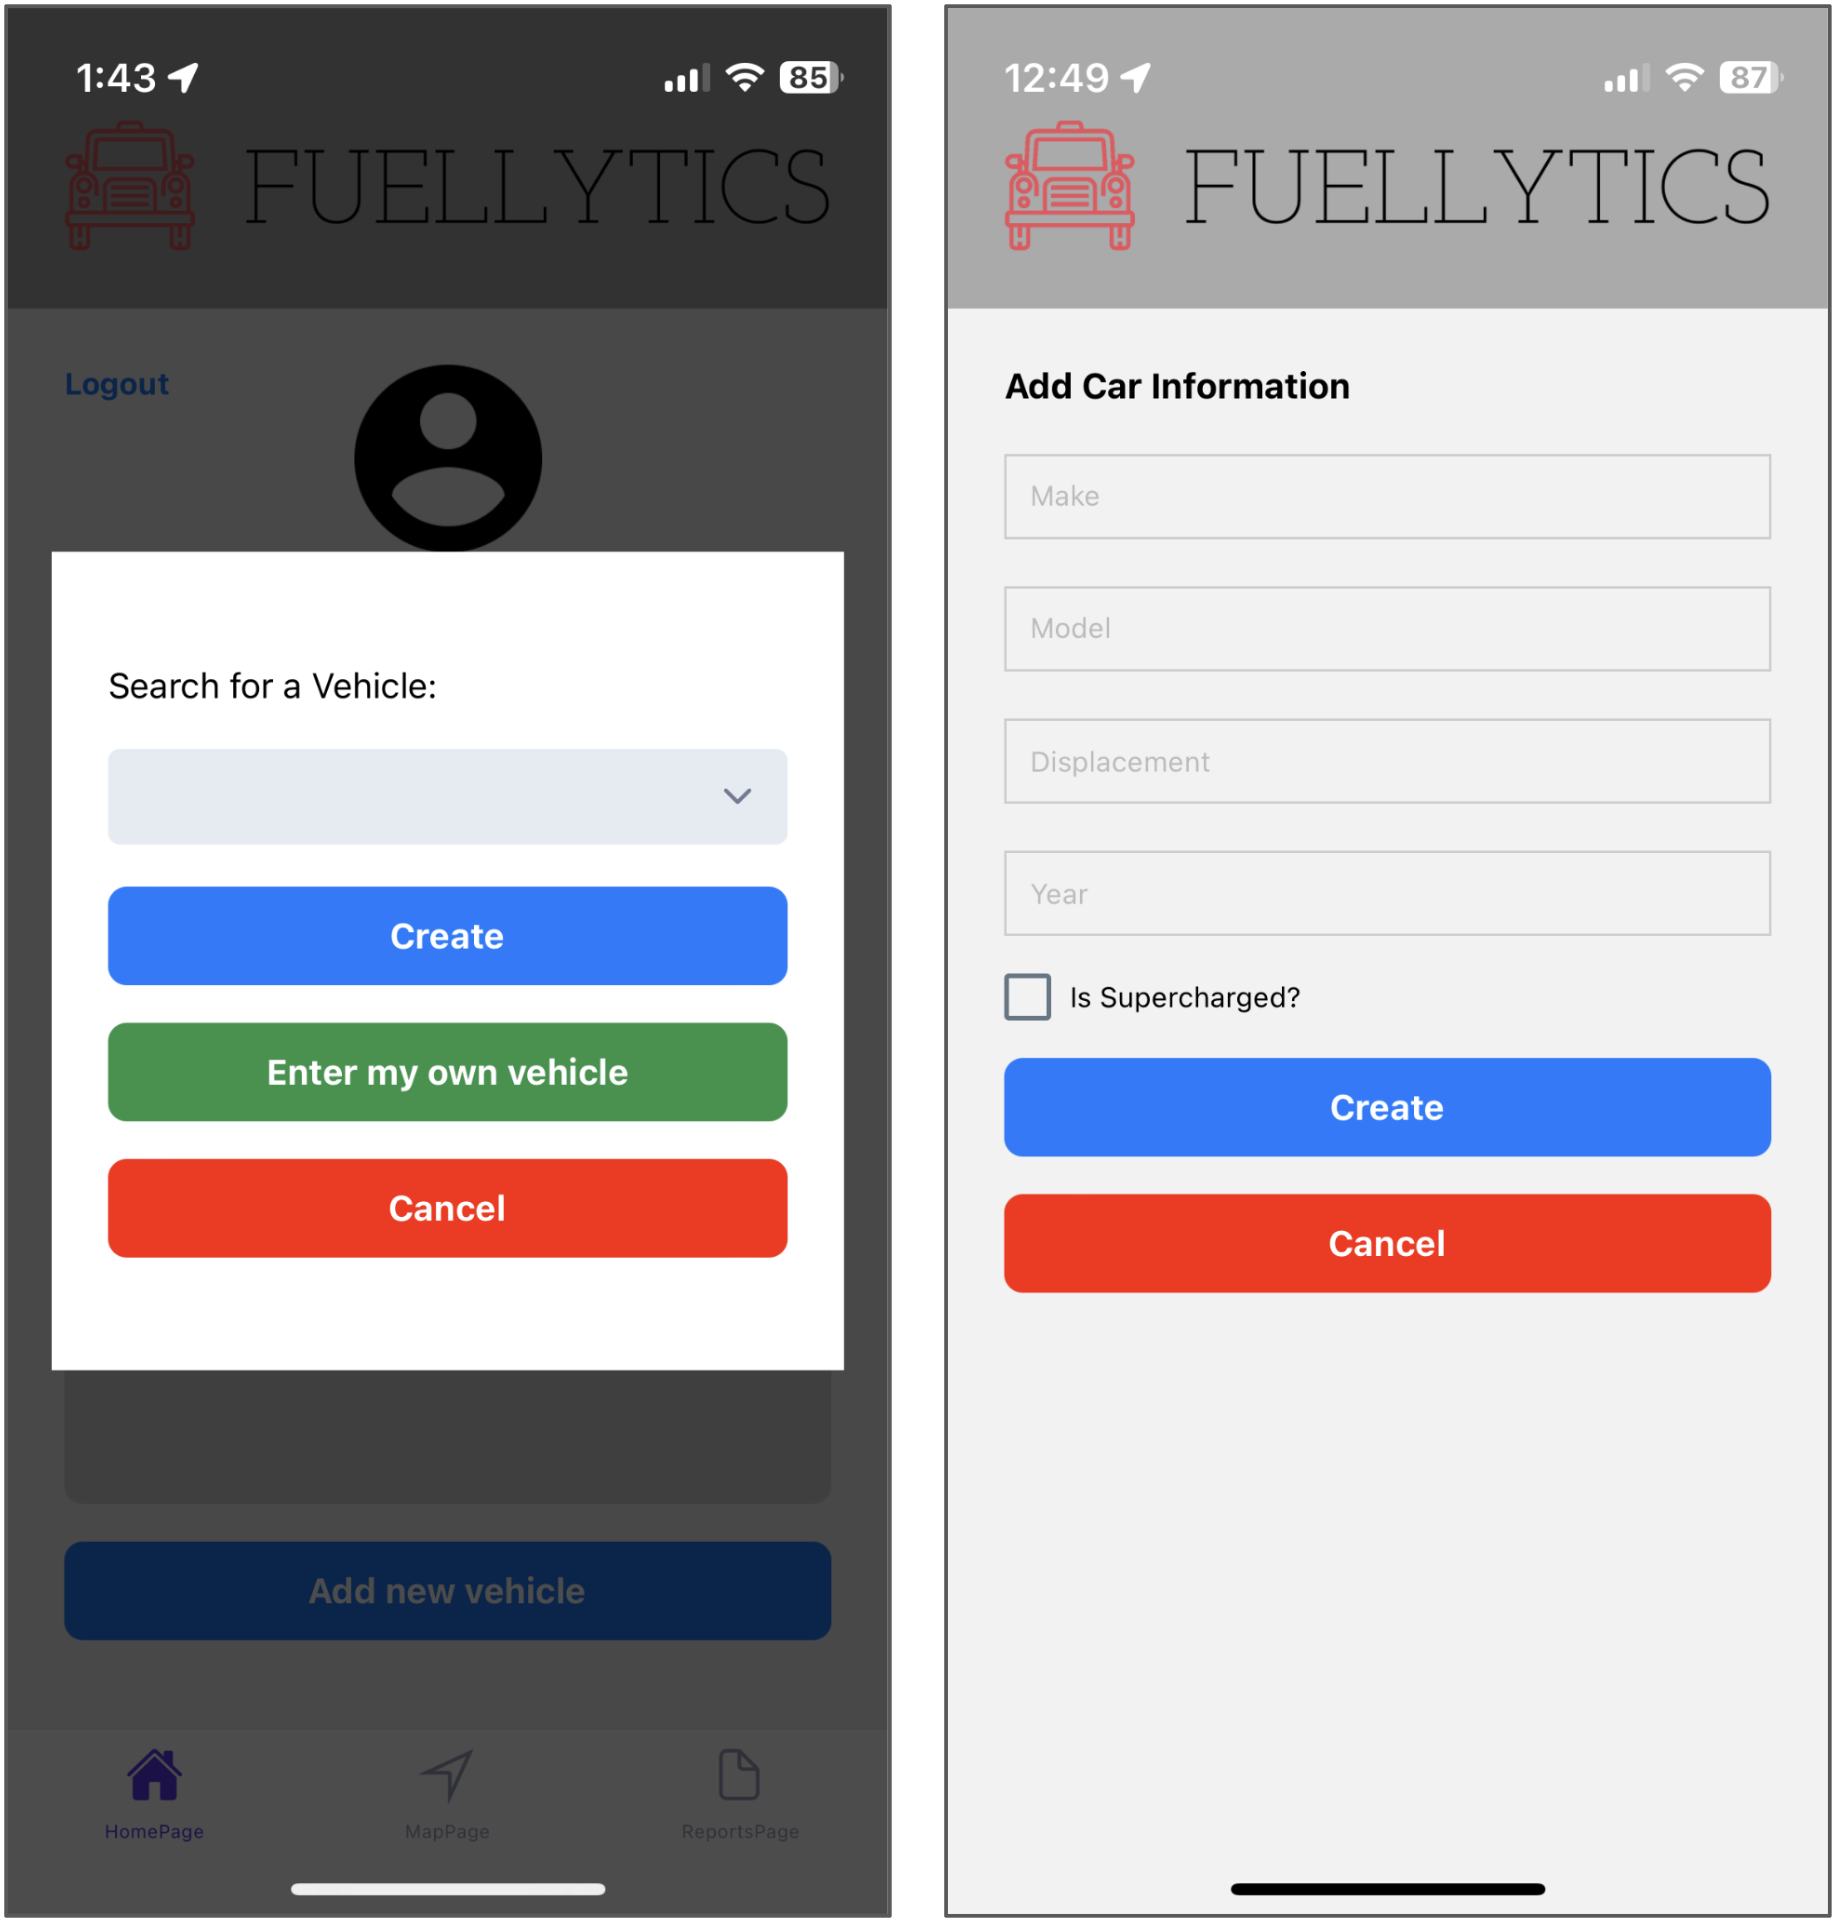
\includegraphics[width=11cm]{img/add-new-vehicle.png}}
\caption{\label{fig:new-vehicle}Popup to add a new vehicle from the Fuellytics database (left), and the window to add a custom vehicle (right).}
\end{figure}

A navigation bar at the bottom of the page allows for easy navigation throughout the Fuellytics application.

The map page, shown in Figure \ref{fig:mappage}, is where users can begin recording their routes and tracking their fuel consumption and carbon emissions.  The user can select their vehicle from the vehicles associated with their account from the dropdown menu.  Initially, the ``Start recording'' button will be hidden and a ``Connecting...'' message will be displayed.  Once the GPS connection has been established and location data is being received, the ``Start recording'' button will become visible, and it will become clickable once a vehicle is selected from the dropdown.

Selecting the ``Start recording'' button will begin a trip recording.  Figure \ref{fig:recording} shows the screens displayed during a trip recording.  These screens contain an interactive map which tracks the user's location in real-time.  A pin is placed on the map showing the users current location, and their track is shown as a black polyline which updates as they move.  A panel slides up from the bottom of the page to reveal plots of the current CO$_2$ emissions of the vehicle in mL/s, the current fuel consumption in mL/s, and the current vehicle speed in km/h.  These plots dynamically update every second, and show data for the last minute.  At any time, the recording can be paused by selecting the ``Pause Recording'' button, and continued by selecting ``Continue Recording''.  
\begin{figure}[!t]
\centerline{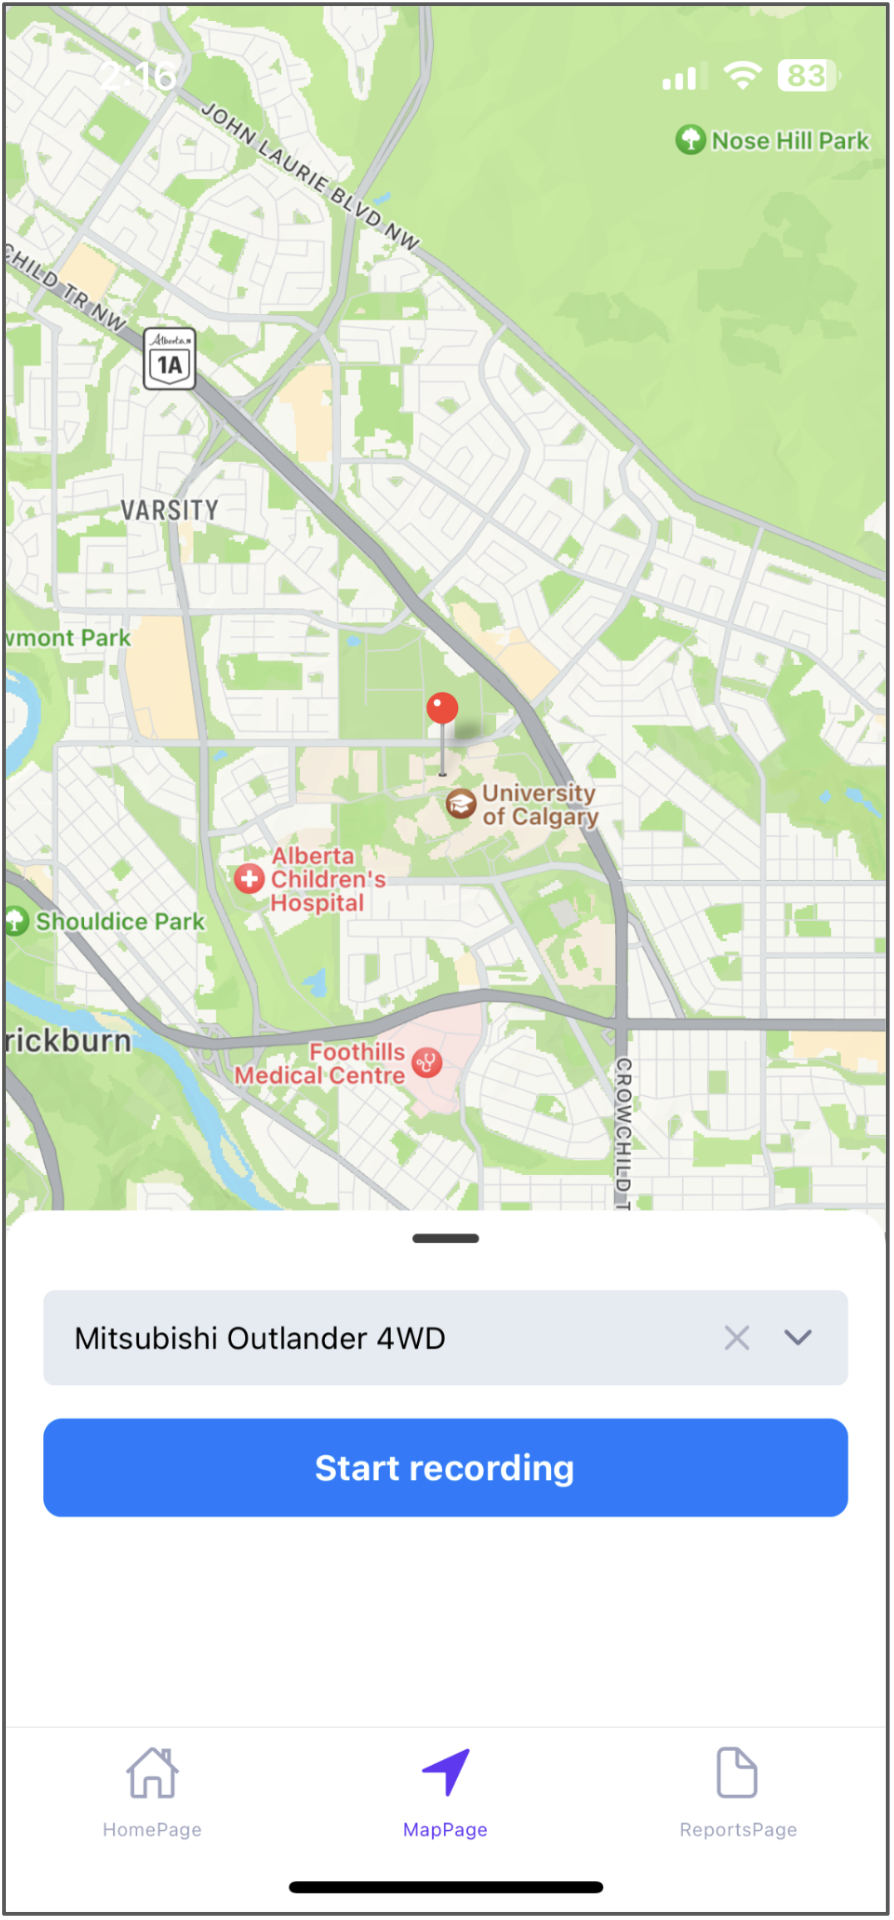
\includegraphics[width=5.5cm]{img/mapinit.png}}
\caption{\label{fig:mappage}The map page where the user can begin a trip recording.}
\end{figure}
\begin{figure}[H]
\centerline{\includegraphics[width=20cm]{img/recording.png}}
\caption{\label{fig:recording}The screens displayed during a trip recording.  From left to right: a map showing the vehicle's location and route, and real-time plots of the CO$_2$ emissions, fuel consumption, and velocity.}
\end{figure}

Once the user arrives at their location, the ``End Recording \& Save'' button will finalize the trip recording and save it.  As shown in Figure \ref{fig:confirmation}, a confirmation page will appear with a summary of the trip including the elapsed time, the total gas consumption, and the total CO$_2$ emissions. Selecting the ``Back'' button brings the user back to the map page.
\begin{figure}[H]
\centerline{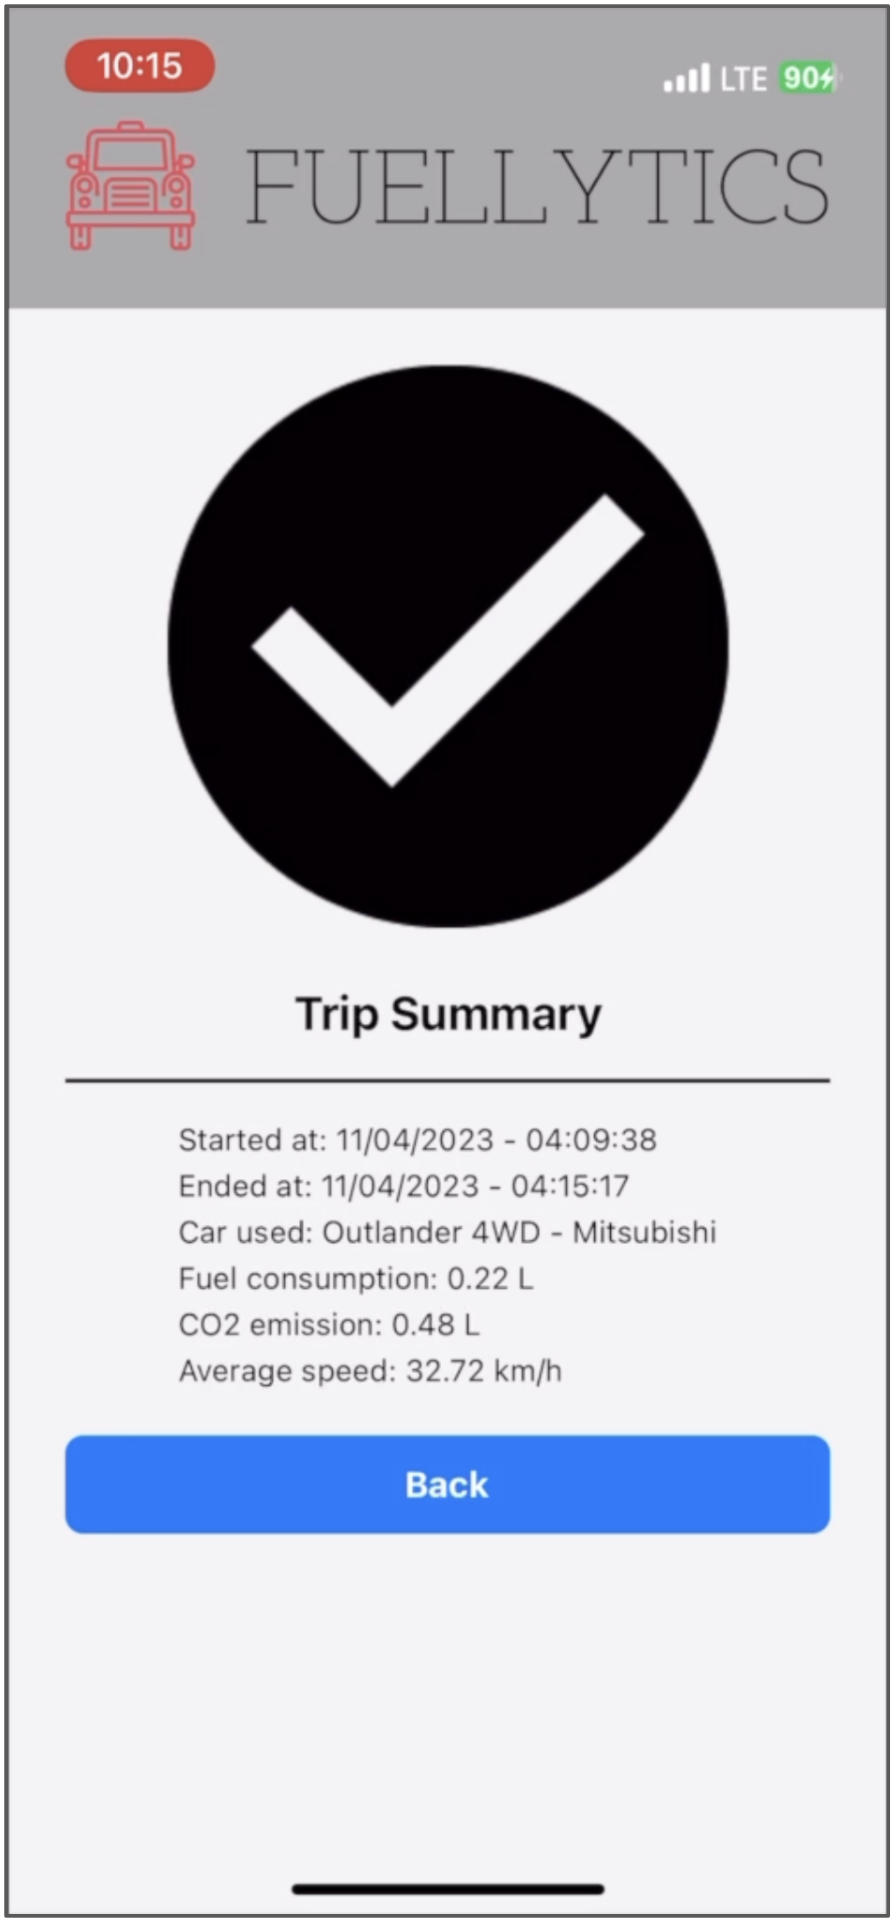
\includegraphics[width=5.5cm]{img/confirmation.png}}
\caption{\label{fig:confirmation}Confirmation page showing a summary of the trip.}
\end{figure}

Summaries of the users trips are available on the reports page, shown in Figure \ref{fig:reports}.  Here, all of the users past trips appear in a scrollable list. The calendar icon above the trip list opens a date range selector widget to filter the trip list within a specified date range. Selecting a trip reveals the trip information page to show further information about the trip including the start and end times, the vehicle used, the total CO$_2$ emissions, the total fuel consumption, and the average speed.  An interactive map is also displayed showing the vehicle route. The user can return to the trips page by selecting the ``Back'' button.
\begin{figure}[H]
\centerline{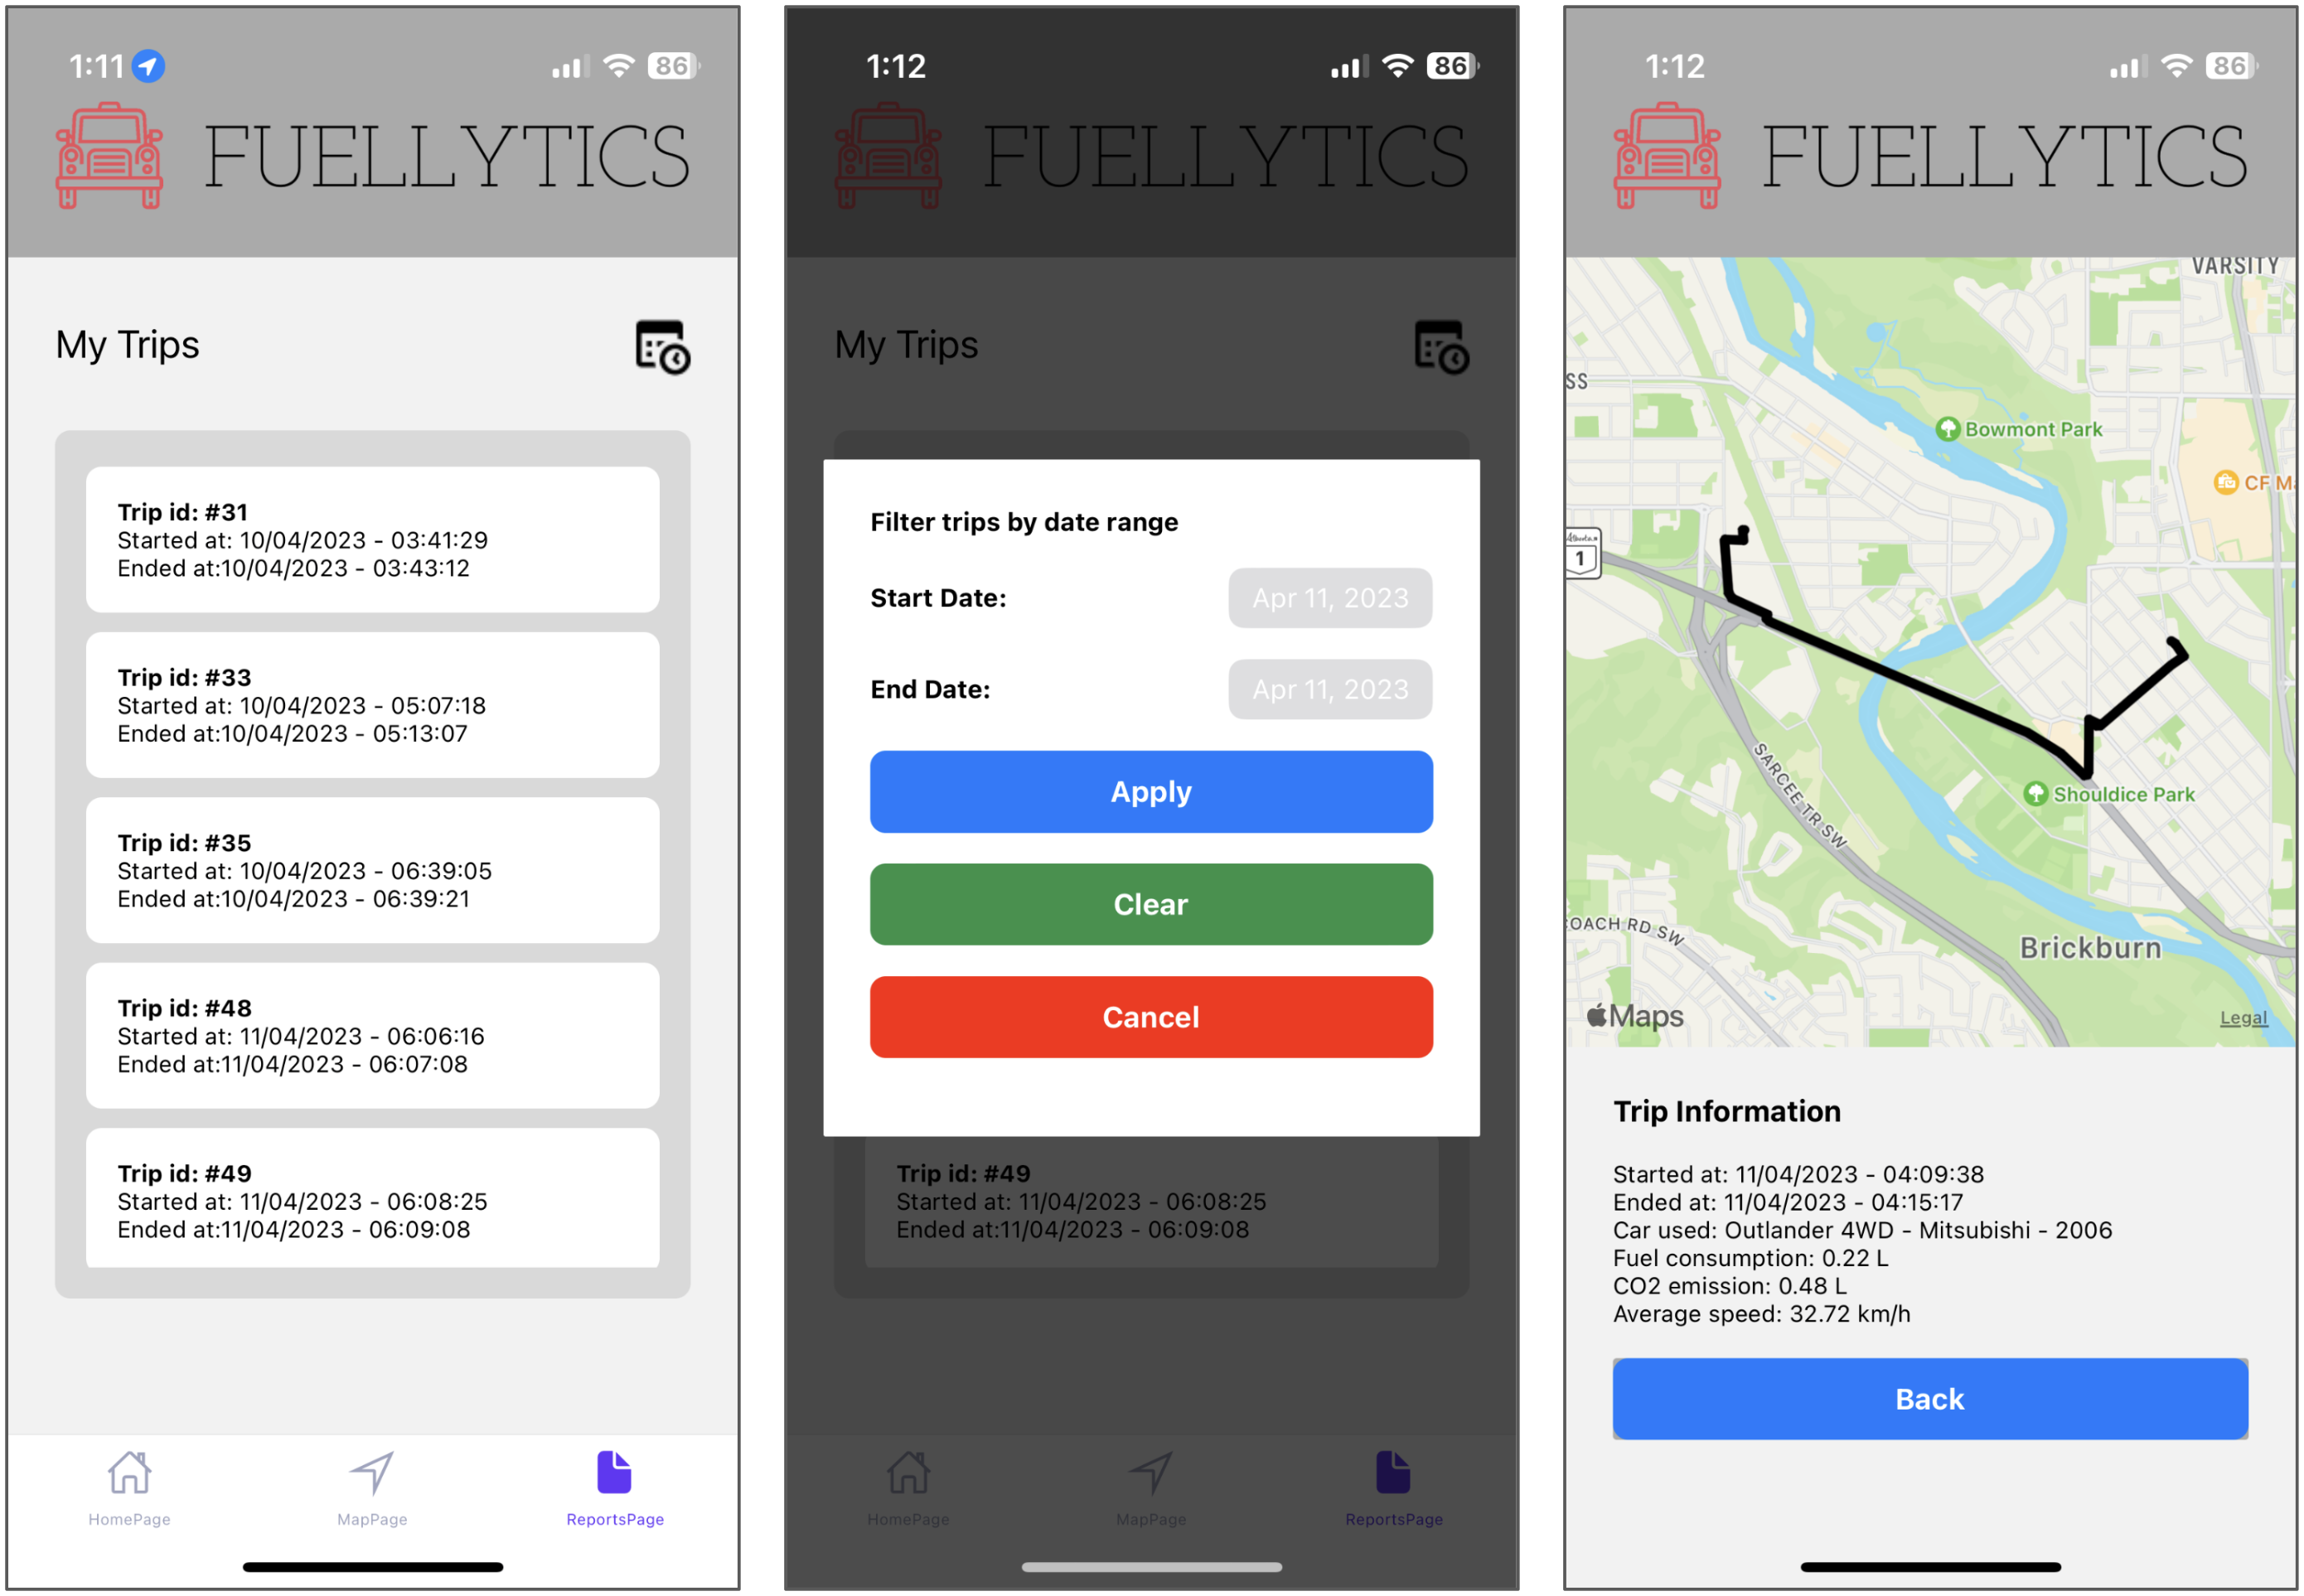
\includegraphics[width=16.5cm]{img/reports.png}}
\caption{\label{fig:reports}The reports page showing all previously logged trips (left), the date filter widget to filter past trips (middle), and the trip information page showing detailed information and a map of the trip.}
\end{figure}

\section{Lessons learned}

One of the most challenging technical aspects of this project was the alignment of the smartphone axes with the frame of the vehicle.  This is necessary to be able to extract the speed, acceleration, and road gradient, which enable the fuel consumption calculation.  Since the smartphone is not fixed in the vehicle and can rotate arbitrarily at any time, the orientation parameters describing the relative vehicle-smartphone orientation must be constantly updated.  The simplest method, and our initial approach, is to utilize the device orientation provided by the iOS and Android operating systems, however, this was found to be unstable and inadequate for our application.  After much testing, our finalized method utilizes the Madgwick AHRS algorithm [\ref*{madgwick}] to combine accelerometer, gyroscope, and magnetometer information and provide orientation of the smartphone with respect to the local level frame.  This is then combined with the GNSS-provided heading to obtain the desired orientation parameters.  This algorithm is fast enough for real-time use, but some inaccuracies arise from the magnetic interference of the metal and electrical components of the vehicle.  As such, it is essential to utilize GNSS-provided navigation parameters to provide corrections to the INS-provided navigation solution.

Several more development-specific lessons were learned during the development process. Notably, it is important to design a real production-grade and scalable architecture that meets current industry standards. This ensures that the application can handle increasing user demand and remains stable over time. Breaking down the project into smaller tasks is also crucial to greatly enhance productivity and make the development process more manageable. Moreover, careful consideration must be given to API design to ensure that the application is functional and performs optimally. It is also crucial to establish a development workflow that prevents conflicts and ensures that team members can work on different repositories simultaneously without major issues. 

The importance of comprehensive testing and performance optimization was also evident during development. Thorough testing helped identify and address bugs and issues before the application was finalized. Meanwhile, optimizing the application for performance, including fast load times and smooth transitions, was critical to providing a positive user experience. By incorporating these lessons learned into the development process, our team was able to create a high-quality application, and the development process ran smoothly and seamlessly, ultimately resulting in a well-fit end product.


\section{Conclusion}
Tracking fuel consumption and carbon emissions from driving is important to understand the efficiency of a vehicle and its environmental impact.  Until now, solutions for an in depth analysis of fuel consumption and carbon emissions have been limited to fleet vehicles in industrial operations, and real-time monitoring of fuel use been presented only in research applications.  The presented smartphone application, \textit{Fuellytics} brings this functionality to the masses.  Fuellytics provides real-time and post-trip analytics of fuel consumption and CO$_2$ emissions in an intuitive and interactive frontend. Moreover, Fuellytics tracks your speed and route to add spatial context to your data.

The project utilized the React Native [\ref*{reactnative}] UI software framework to enable simplified development and cross-platform compatibility, and the Python-based web framework Django [\ref*{django}] to provide a functional and reliable backend.  Careful consideration of the architecture was done to ensure reliability, scalability, and ease of development. Several AWS [\ref*{aws}] services, including Elastic Load Balancer, Elastic Compute Cloud, Relational Database Service, Simple Storage Service, Lambda, and CloudWatch were utilized to host the application and provide a functional and dependable platform.

Through the development of Fuellytics, our team gained valuable experience in geospatial web development, mobile development and interaction with IoT sensors.  We faced various technical challenges, such as accurately aligning the smartphone axes with the vehicle frame and designing a scalable architecture that meets industry standards. However, by utilizing industry-standard development practices, breaking down the project into smaller tasks, and implementing comprehensive testing and performance optimization, we were able to overcome these challenges and create a high-quality application.

Overall, Fuellytics represents a significant contribution to the field of vehicle fuel efficiency, offering users real-time data and insights that can help them optimize their driving habits and reduce their fuel consumption. We believe that this application has the potential to make a meaningful impact on the environment and the economy, and we are hopeful to see it being used by individuals and organizations in the near future.

\section{LLM usage}
Two openly available large language models, namely ChatGPT \reflabel{chatgpt} and Open Assistant \reflabel{open-assistant}, were used at various stages of this project. ChatGPT was a valuable resource in developing the Fuellytics codebase, providing suggestions for debugging and bug fixes, as well as offering guidance on coding practices.  In addition, both ChatGPT and Open Assistant assisted in the creation of this report, helping to improve the grammar and sentence structure and transforming bullet points into coherent paragraphs. These LLM's proved to be powerful tools for enhancing both the development and written communication aspects of the project.

\section{References}

\begin{footnotesize}

\refinit{canadaghg} ``Greenhouse Gas Emissions: Canadian Environmental Sustainability Indicators,'' \textit{Environment and Climate Change Canada}, 2022. Available: \url{https://www.canada.ca/en/environment-climate-change/services/environmental-indicators/greenhouse-gas-emissions.html}

\refinit{reactnative} React-Native, \textit{Meta Platforms, Inc.}, \url{https://reactnative.dev}

\refinit{django} Django, \textit{Django Software Foundation}, \url{https://www.djangoproject.com}

\refinit{aws} Amazon Web Services, \url{https://aws.amazon.com}

\refinit{transport-emissions} ``Transport, Energy and CO2,'' \textit{International Energy Agency}, Paris, France, 2009. Available: \url{https://www.iea.org/reports/transport-energy-and-co2}

\refinit{oil-based-transport} ``Transport,'' \textit{International Energy Agency}, Paris, France, 2022. Available: \url{https://www.iea.org/reports/transport}

\refinit{driving-style} ``Techniques for Drivers to Conserve Fuel,'' \textit{U.S. Department of Energy}, \url{https://afdc.energy.gov/conserve/behavior_techniques.html}

\refinit{fuel-force} FuelForce Fuel Management Systems, \textit{Multiforce Systems}, \url{https://info.gartnerdigitalmarkets.com/multiforce-gdm-lp?channel=capterra}

\refinit{triscan} Triscan Systems, \textit{Triscan Group Limited}, \url{https://www.thetriscangroup.com}

\refinit{fuelly} Fuelly, \textit{Fuelly, LLC}, \url{https://www.fuelly.com}

\refinit{fuelline} C. Olafson, E. Johston, B. Masciotra, and Y. Mo. \textit{FuelLine}, \url{https://fuel-line.fly.dev/}

\refinit{myearth} ``MyEarth - Track carbon savings,'' \textit{University of Wisconsin}, \url{https://play.google.com/store/apps/details?id=com.ionicframework.myearthapp496614&hl=en_CA&gl=US}

\refinit{capture} ``Carbon Footprint \& CO2 Tracker,'' \textit{The Capture Club}, \url{https://play.google.com/store/apps/dev?id=7417037584465272817&hl=en_CA&gl=US}

\refinit{main-paper}  Q. Zhao, Q. Chen, and L. Wang. ``Real-Time Prediction of Fuel Consumption Based on Digital Map API,'' \textit{Applied Sciences}, vol. 9, no. 7, p. 1396, 2019. \url{https://doi.org/10.3390/app9071369}

\refinit{tank2wheel} C. M. Silva, G. A. Goncalves, T. L. Farias, and J. M. C. Mendes-Lopes. ``A tank-to-wheel analysis tool for energy and emissions studies in road vehicles,'' \textit{Science of The Total Environment}, vol. 367, no. 1, pp. 441-447, 2006. \url{https://doi.org/10.1016/j.scitotenv.2006.02.020}

\refinit{analytic-fc} M. Ben-Chaim, E. Shmerling, and A. Kuperman. ``Analytic Modeling of Vehicle Fuel Consumption,'' \textit{Energies}, vol. 6, no. 1, pp. 117-127, 2013. \url{https://doi.org/10.3390/en6010117}

\refinit{wvu-ai} S. Katreddi and A. Thiruvengadam. ``Trip Based Modeling of Fuel Consumption in Modern Heavy-Duty Vehicles Using Artificial Intelligence,'' \textit{Energies}, vol. 14, no. 24, p. 8592, 2021. \url{https://doi.org/10.3390/en14248592}

\refinit{fc-phone} Y. Yao, X. Zhao, C. Liu, J. Rong, Y. Zhang, Z. Dong, and Y. Su. ``Vehicle Fuel Consumption Prediction Method Based on Driving Behavior Data Collected from Smartphones,'' \textit{Journal of Advanced Transportation}, vol. 2020, 2020. \url{https://doi.org/10.1155/2020/9263605}

\refinit{madgwick} S. O. H. Madgwick. ``AHRS algorithms and calibration solutions to facilitate new applications using low-cost MEMS,'' Ph. D. dissertation, University of Bristol, England, 2014. Available: \url{https://ethos.bl.uk/OrderDetails.do?uin=uk.bl.ethos.681552}

\refinit{chatgpt} ChatGPT, \textit{OpenAI}, 2023. \url{https://openai.com/blog/chatgpt}

\refinit{open-assistant} Open Assistant, 2023. \url{https://open-assistant.io}

\end{footnotesize}


\end{document}
